\tikzstyle{n}=[xshift=.3cm, yshift=.3cm]
\tikzstyle{a}=[red]
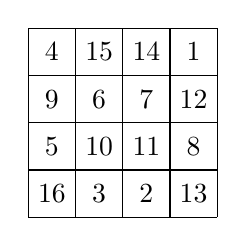
\begin{tikzpicture}[scale=.6]
  %\foreach\i in {0,1,2,3}{
  %  \draw[a] (.1, {0 + .5}) -- ++(4.2, 0);
  %  \draw[a] ({0 + .5}, .1) -- ++(0, 4.2);
  %}

  \draw (0, 0) grid (4, 4);
  \node[n] at (0, 0) {16};
  \node[n] at (1, 0) {3};
  \node[n] at (2, 0) {2};
  \node[n] at (3, 0) {13};

  \node[n] at (0, 1) {5};
  \node[n] at (1, 1) {10};
  \node[n] at (2, 1) {11};
  \node[n] at (3, 1) {8};

  \node[n] at (0, 2) {9};
  \node[n] at (1, 2) {6};
  \node[n] at (2, 2) {7};
  \node[n] at (3, 2) {12};

  \node[n] at (0, 3) {4};
  \node[n] at (1, 3) {15};
  \node[n] at (2, 3) {14};
  \node[n] at (3, 3) {1};

  %\foreach\i in {0,1,2,3}{
  %  \node[n, a] at (4,  \i) { 34};
  %  \node[n, a] at (\i, -1) { 34};
  %}
  %\node[n, a] at (4, 4) { 34};
  %\node[n, a] at (4, -1) { 34};

\end{tikzpicture}
